%!TEX encoding = UTF-8 Unicode
%!TEX root = ../compendium2.tex

\section{JetBrains IntelliJ IDEA med Scala-plugin}\label{appendix:ide:intellij}

IntelliJ IDEA%
\footnote{\href{https://en.wikipedia.org/wiki/IntelliJ_IDEA}{en.wikipedia.org/wiki/IntelliJ\_IDEA}}
 är en professionell IDE som stödjer många olika programmeringsspråk. IntelliJ är skriven i Java och utvecklas av det tjeckiska företaget JetBrains.

IntelliJ IDEA finns i två varianter: en gratis gemenskapsvariant med öppenkällkodslicens \Eng{Community edition}, samt en betalvariant med sluten källkod och support-tjänster.


IntelliJ IDEA är en omfattande och avancerad programmeringsmiljö med många funktioner och inställningar. Det finns även en omfattande uppsättning insticksmoduler och tilläggsprogram som underlättar utveckling av t.ex. mobilappar, webbprogram, databaser och mycket annat.

Till IntelliJ IDEA finns en insticksmodul \Eng{plug-in} som stöd för Scala med tillhörande standardbibliotek och byggverktyget \code{sbt}, med mera. Scala-insticksmodulen kan inkluderas genom att välja Scala i en av de dialoger som visas vid första körningen, enligt instruktioner nedan.

I detta avsnitt ges länkar till installation samt tips om hur du kommer igång med att använda IntelliJ IDEA med Scala. Det går ganska snabbt att lära sig grunderna, men det kräven en viss ansträngning att lära sig de mer avancerade funktionerna. Det finns omfattande resurser på nätet som hjälper dig vidare.

Google tillkännagav 2013 att företaget övergår från Eclipse till IntelliJ som den officiellt understödda utvecklingsmiljön för Android och 2014 lanserades utvecklingsmiljön Android Studio%
\footnote {\href{https://en.wikipedia.org/wiki/Android_Studio}{en.wikipedia.org/wiki/Android\_Studio}}
 som bygger vidare på IntelliJ.

\subsection{Installera IntelliJ IDEA}\label{appendix:ide:intellij:install}

IntelliJ med Scala-plug-in är förinstallerat på LTH:s datorer och startas med kommandot \texttt{idea} i ett terminalfönster.

\begin{itemize}
\item För Ubuntu Linux finns ett färdigt paket som du kan installera med dessa kommandon i terminalen:
\begin{REPLnonum}
sudo add-apt-repository ppa:mmk2410/intellij-idea-community
sudo apt-get update
sudo apt-get install intellij-idea-community
sudo apt-get upgrade
sudo ln -s /opt/intellij-idea-community/bin/idea.sh /usr/local/bin/idea
\end{REPLnonum}
Det sista kommandot är inte nödvändigt men ger samma startkommando som på skolans datorer. Du kan även starta \textit{IntelliJIDEA Community Edition} via startmenyn genom att söka på intellij.
Mer information om denna ppa finns här:\\ \url{https://launchpad.net/~mmk2410/+archive/ubuntu/intellij-idea-community}\item För Windows och Mac: ladda ner och kör installationsfil för ditt operativsystem för den öppna varianten kallad \textbf{Community} här: \\
\url{https://www.jetbrains.com/idea/download/} \\
Följ instruktionerna som ges av installationsprogrammet.
\end{itemize}

\subsection{Anpassa IntelliJ IDEA och installera Scala-plugin}\label{appendix:ide:intellij:tweak}
Första gången du kör igång IntelliJ får du ett antal frågor om vilka anpassningar du vill göra. Följ instruktionerna steg för steg enligt nedan.
\begin{enumerate}

\item Först visas en dialog med titeln \textbf{Complete Installation} som frågar dig om du eventuellt vill importera gamla inställningar eller köra igång med en installation från grunden:
\begin{figure}[H]
\centering
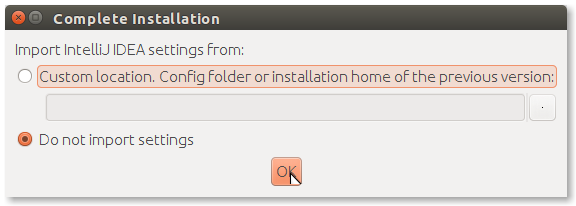
\includegraphics[width=0.75\textwidth]{../img/intellij/idea1-complete-installation.png}
\caption {Första gången får du denna dialog. Klicka \Button{Ok}.}
\label{fig:eclipse:import-projects}
\end{figure}
Om du inte får denna dialog har du troligen en dold katalog i din hemkatalog från en tidigare installation som börjar med namnet \texttt{.Idea} följt av versionnummer. Om du tar bort denna katalog före du kör igång IntelliJ kan du göra om inställningarna från grunden.

\item Efter licensacceptansdialogen kommer fönstret \textbf{Custumize IntelliJ IDEA} där du först får välja att ställa in \textbf{UI Theme}. Denna inställning gäller utseende på gränssnittet. Det tema som kallas \textit{Darcula} är en populär variant med mörk bakgrund och nedtonade färger anpassade för att vara skonsamma mot ögonen. Du kan lätt ändra detta val senare. Klicka \Button{Next} när du valt tema.

\item Därefter kan du i fönstret \textbf{Custumize IntelliJ IDEA} välja att installera skrivbordsikon och startmenyikon och sedan att skapa ett körskript. Om du kör Linux och installerat IntelliJ enligt föregående avsnitt eller kör på LTH:S datorer har du redan detta och du kan med fördel \textbf{avmarkera dessa val om ikon och startskript} och slippa dubbla ikoner i startmenyn. Kör du Windows eller MacOS kan du i stället med fördel välja installation av startikoner och startskript.

\item \textbf{Default plugins:} \emph{Tune IDEA to your tasks}. Denna dialog gäller inställningar av befintliga insticksmoduler. Dessa inställningar fungerar bra som de är. Klicka \Button{Next}.

\item \textbf{Featured plugins}. I rutan för \textbf{Plugin for Scala language support} Klicka \Button{Install} och låt installationen av Scala fullbordas.

\item När Scala-plugin-installationen är klar, klicka \Button{Start using IntelliJ IDEA}.

\item I välkomstfönstrets nedre hörn, välj \MenuArrow{Configure}\Menu{Settings} och överväg om du vill göra följande lämpliga men ej nödvändiga inställningar.
\begin{enumerate}
\item I fliken \MenuArrow{Editor}\Menu{General} markera \FramedCheckmark{Change font size (Zoom) with Ctrl+Mouse Wheel} för att lätt kunna ändra textstorlek i editorn. Glöm inte att klicka \Button{Apply} nere till höger.

\item I fliken \MenuArrow{Editor}\Menu{Inspections} och välj att expandera \Menu{Spelling} i högra listan. Avmarkera \FramedUnchecked{Typo} för att undvika att svenska ord blir markerade som felstavade. Glöm inte att klicka \Button{Apply} nere till höger.

\item I fliken \MenuArrow{Editor}\Menu{File and Code Templates} och under fliken \Menu{Files} i högra listan: för varje Scala-filtyp (Scala Class, Scala Trait, Scala Object, ...) ta bort andra raden i mallen med texten \code{#parse("File Header.java")} för att slippa onödiga kommentarer i koden när du skapar nya filer. Glöm inte att klicka \Button{Apply} nere till höger. Klicka OK när du är klar med att ändra i \Menu{Settings}.

\end{enumerate}
\end{enumerate}
Du kan också göra ovan och liknande anpassningar senare genom applikationsmenyn \MenuArrow{File}\Menu{Settings...}. Det finns en enorm mängd inställnigar som du kan läsa om i hjälpen som finns på Jetbrains hemsida. Om du vill tillbaka till grundinställningarna kan du ta bort den dolda katalog i din hemkatalog som börjar med namnet \texttt{.Idea} följt av versionnummer och börja om i grundläge vid nästa applikationsstart.





\subsection{Använda IntelliJ IDEA med Scala-plugin}%\label{appendix:ide:intellij:use}

\subsubsection{Skapa ett nytt Scala-projekt}

När du startar IntelliJ IDEA utan förvalt projekt visas välkomstskärmen i figur \ref{fig:idea:welcome}.
\begin{figure}[H]
\centering
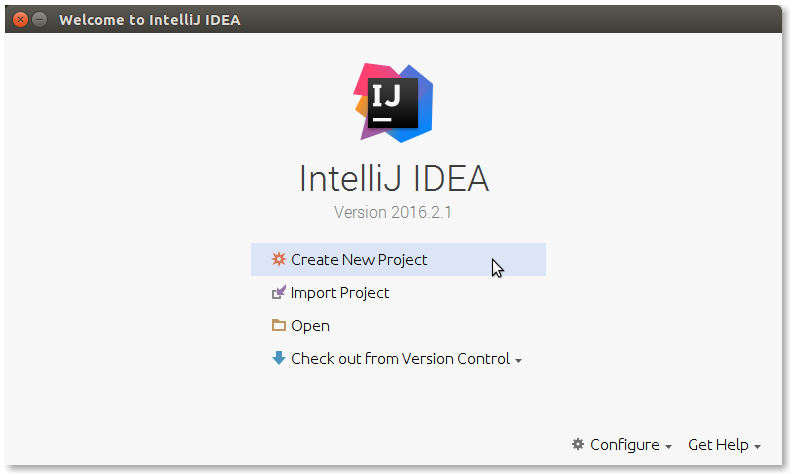
\includegraphics[width=1.0\textwidth]{../img/intellij/idea-welcome.png}
\label{fig:idea:welcome}
\caption{Välkomstfönstret för IntelliJ IDEA.}
\end{figure}

\noindent Klicka på \Menu{Create New Project}, varefter dialogen i figur \ref{fig:idea:new-project} visas. Följ stegen enligt nedan.


\begin{enumerate}
\item I dialogen \textbf{New Project} ska du välja projekttyp och körmiljö för ditt projekt enligt figur \ref{fig:idea:new-project}. Välj Scala och SBT och klicka \Button{Next}.

\item Ge projektet namnet \texttt{hello} enligt figur \ref{fig:idea:new-hello-project}.

\begin{figure}[H]
\centering
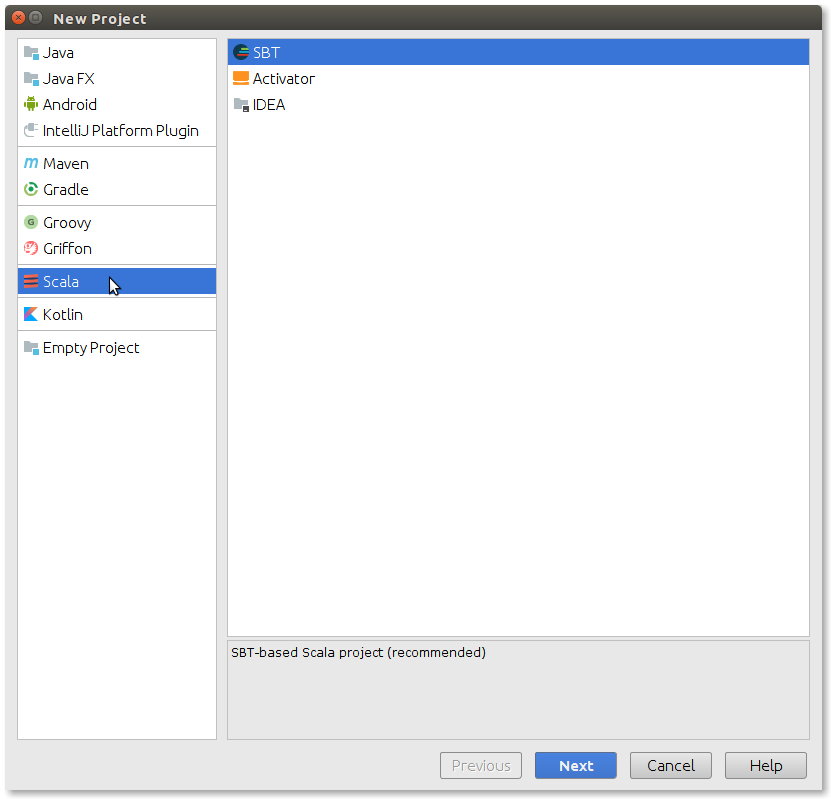
\includegraphics[width=1.0\textwidth]{../img/intellij/idea-new-scala-project.png}
\caption{Välj att skapa ett Scala-projekt med SBT och klicka \Button{Next}.}
\label{fig:idea:new-scala-project}
\end{figure}

\begin{figure}[H]
\centering
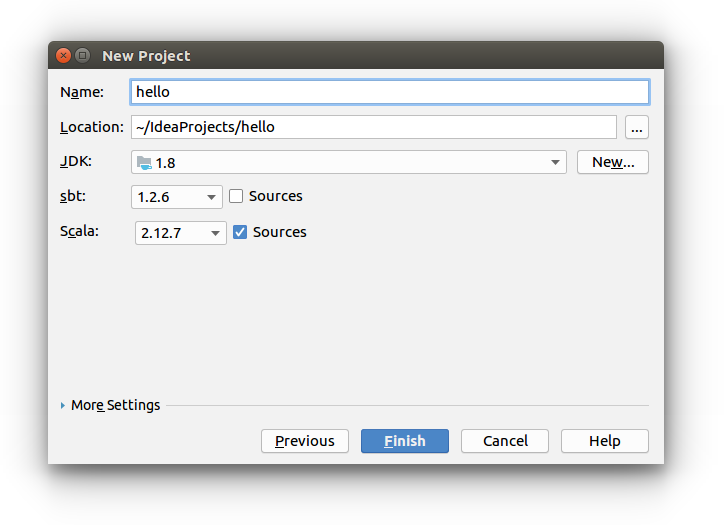
\includegraphics[width=1.0\textwidth]{../img/intellij/idea-new-hello-project.png}
\caption{Ge ditt nya Scala-projekt ett namn.}
\label{fig:idea:new-hello-project}
\end{figure}

\item Avsluta med att klicka \Button{Finish}.

\item Nu öppnas ett projektfönster och det visas även ett välkomstfönster \textit{Tip of the Day} med tips om hur du använder IntelliJ (om du inte stängt av denna funktion). Om du vill kan du läsa igenom några tips nu, eller så kan du stänga fönstret och läsa tipsen nästa gång du öppnar/skapar ett projekt. Tipsen är en god hjälp att komma igång med alla kortkommandon som gör ditt arbete effektivt. %Projektfönstret visas i figur \ref{fig:idea:project-hello}..

% \begin{figure}[H]
% \centering
% 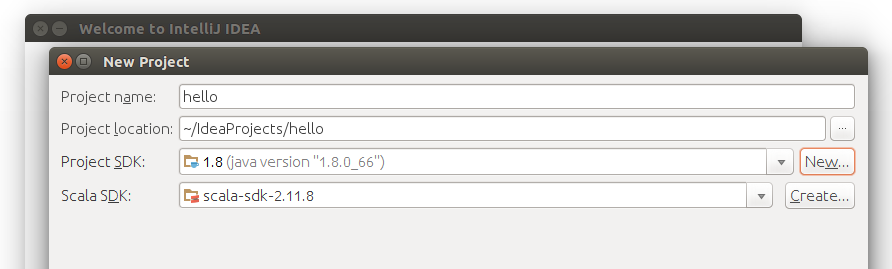
\includegraphics[width=1.0\textwidth]{../img/intellij/idea-new-project.png}
%
% \begin{minipage}{0.27\textwidth}
% 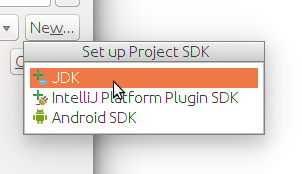
\includegraphics[width=1.0\textwidth]{../img/intellij/idea-project-sdk-jvm.png}
% \end{minipage}
% \begin{minipage}{0.35\textwidth}
% 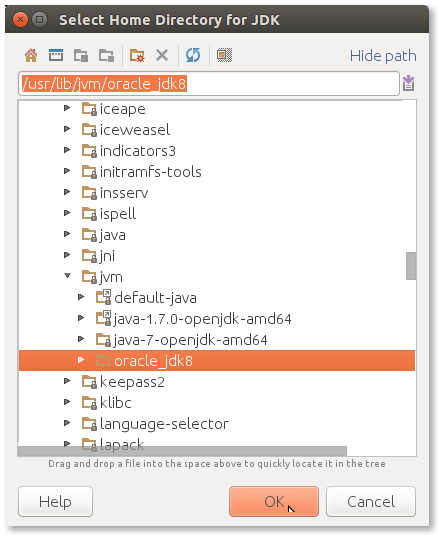
\includegraphics[width=1.0\textwidth]{../img/intellij/idea-project-sdk-home.png}
% \end{minipage}
% \begin{minipage}{0.35\textwidth}
% 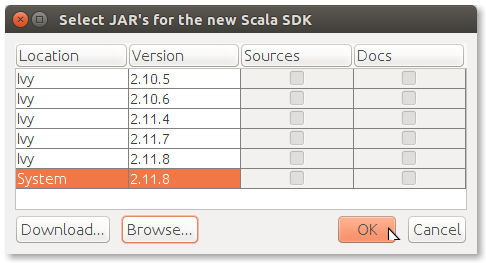
\includegraphics[width=1.0\textwidth]{../img/intellij/idea-scala-sdk.png}
% \end{minipage}%
%
% \caption{Namnge ditt projekt och ställ in körmiljön för JVM och Scala genom att klicka på \Button{New...} och \Button{Create...}}.
% \label{fig:idea:new-project}
% \end{figure}



\begin{figure}
\centering
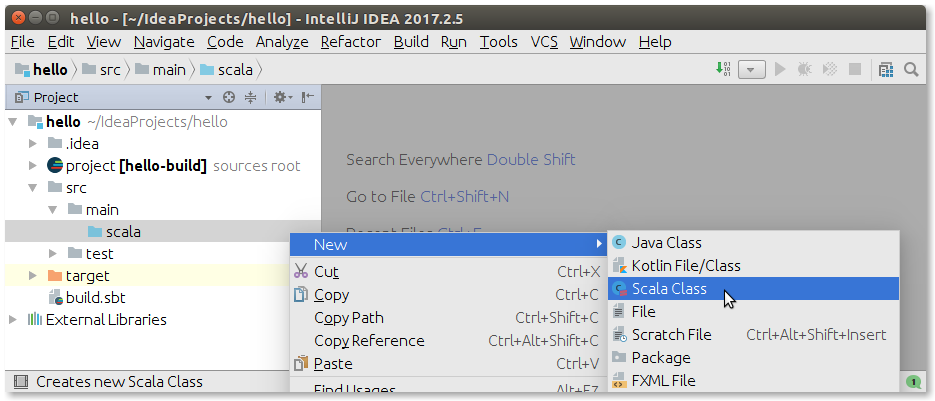
\includegraphics[width=1.0\textwidth]{../img/intellij/idea-new-scala-class.png}

\begin{minipage}{0.35\textwidth}
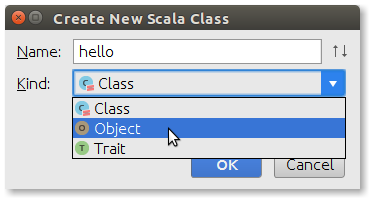
\includegraphics[width=1.0\textwidth]{../img/intellij/idea-scala-object.png}
\end{minipage}
\begin{minipage}{0.60\textwidth}
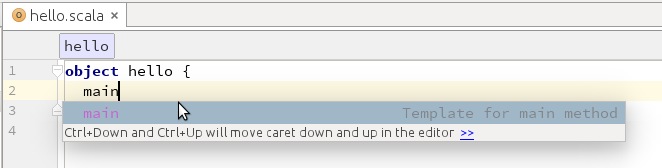
\includegraphics[width=1.0\textwidth]{../img/intellij/idea-complete-main.png}
\end{minipage}%

\caption{Välj \MenuArrow{New}\Menu{Scala Class} genom att högerklicka på  mappen \texttt{src/main/scala} och skapa ett nytt Scala-objekt med \code{main}-metod. Aktivera kodkomplettering i editorn efter ordet \code{main} genom att trycka på TAB-tangenten.}
\label{fig:idea:project-hello}
\end{figure}


\item Klicka på projektmappen \code{hello} och veckla ut mappen \texttt{src/main/scala} och högerklicka på \texttt{scala}-mappen och välj \MenuArrow{New}\Menu{Scala Class}.Välj sedan \textbf{Object} i dialogen \textbf{Create New Scala Class} och klicka \Button{OK}, enligt figur \ref{fig:idea:project-hello}.

\item Du får nu upp ett editorfönster med koden för objektet \code{hello}. Skriv ordet \code{main} inuti objektet och tryck TAB för att aktivera kodkomplettering. En mall för \code{main}-metoden klistras då in i objektet.

\item Skriv kod så att det ser ut som i editorfönstret i figur \ref{fig:idea:hello-world} på sidan \pageref{fig:idea:hello-world}.

\item \textbf{Bakgrundsaktiviteter}. Nere i projektföntrets statusområde visas aktiviteter, t.ex. nedladdningar och kompileringar, som pågår i bakgrunden. Du kan ofta arbeta med editering parallellt med bakgrundsaktiviteter, men t.ex. vid körning av program behöver du ibland vänta tills bakgrundsaktiviteterna är klara. Det kan därför vara bra att hålla koll på progress av bakgrundsaktiviteter om du undrar varför du ibland inte får omedelbar respons.


\item Kör igång ditt program genom att klicka på play-knappen eller genom att trycka Shift+F10. Om play-knappen är initialt är grå i stället för grön, välj menyn \MenuArrow{Run}\Menu{Run...}.

\end{enumerate}


\noindent Mer information om hur du använder Scala-plugin för IntelliJ finns här:\\
\href{https://confluence.jetbrains.com/display/SCA/Scala+Plugin+for+IntelliJ+IDEA}{confluence.jetbrains.com/display/SCA/Scala+Plugin+for+IntelliJ+IDEA}

\begin{figure}
\centering
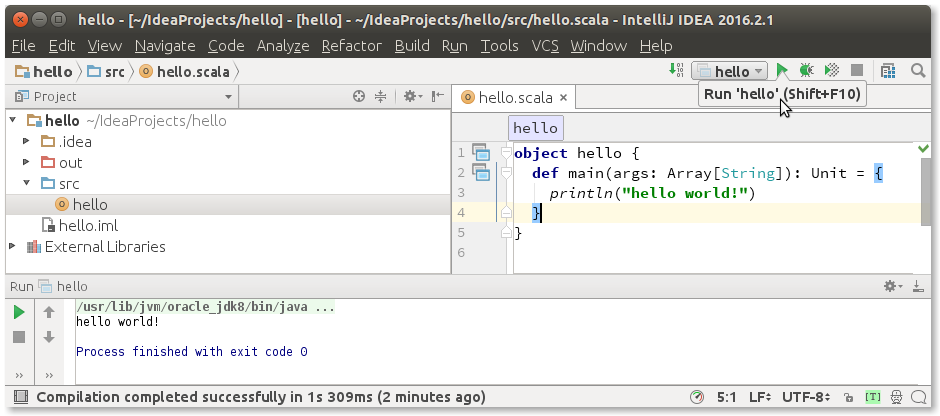
\includegraphics[width=1.0\textwidth]{../img/intellij/idea-hello.png}
\caption{Kör ditt program med play-knappen eller (första gången) välj menyn \MenuArrow{Run}\Menu{Run...} och välj \code{hello}.}
\label{fig:idea:hello-world}
\end{figure}


\subsubsection{Ladda ner kursens workspace och importera i IntelliJ IDEA}

Det finns en zip-fil med ett workspace med projekt för flera av kursens laborationer som du kan ladda ner och importera i Eclipse. Följ stegen nedan.

\begin{enumerate}
\item Ladda ner kursens workspace här: \url{http://cs.lth.se/pgk/ws}

\item Packa upp filen på lämpligt ställe.

\item Starta IntelliJ. Om du redan har ett projekt igång välj menyn \MenuArrow{File}\Menu{Close project} så kommer du tillbaka till välkomstfönstret. Välj \textbf{Import Project} så som visas i figure \ref{fig:idea:import1-project}.

\begin{figure}[H]
\centering
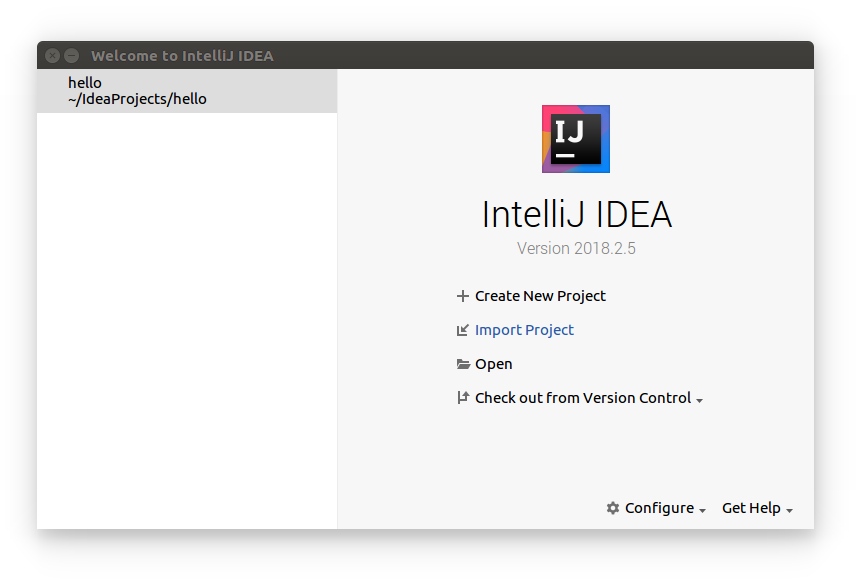
\includegraphics[width=1.0\textwidth]{../img/intellij/idea-import1-project.png}
\caption{Välj \Menu{Import Project} efter att du stängt ev. öppna projekt.}
\label{fig:idea:import1-project}
\end{figure}

\item Bläddra dit du packat upp workspace och markera denna folder i likhet med figur \ref{fig:idea:import23-select} och klicka \Button{OK}. I den efterföljande dialogen välj \textbf{Eclipse} och klicka \Button{Next}.

\item Klicka \Button{Next} igen i dialogen som liknar figur \ref{fig:idea:import4-directory} på sidan \pageref{fig:idea:import4-directory}, där mappen du valt är förvald.

\item Klicka \Button{Next} igen enligt figur \ref{fig:idea:import5-select-projects} på sidan  \pageref{fig:idea:import5-select-projects}. Alla tillgängliga Eclipse-projekt ska vara markerade.

\item Klicka \Button{Finish} enligt figur \ref{fig:idea:import5-select-projects} med förifylld text oförändrad.

\item Bläddra fram filen \texttt{PirateSpeech.scala} och öppna den med ett dubbelklick. Klicka på länken \textbf{Setup Scala SDK} uppe till höger enligt figur \ref{fig:idea:import78-setup-scala-sdk} på sidan \pageref{fig:idea:import78-setup-scala-sdk}. I efterföljande dialog kontrollera att \texttt{scala-sdk-2.11.8} är förvalt och klicka \Button{OK}.

\item Lägg till testutskrift enligt rad 7 i figur \ref{fig:idea:import9-run} på sidan \pageref{fig:idea:import9-run}. Testkör genom att välja menyn \MenuArrow{Run}\Menu{Run..} eller tryck Alt+Shift+F10 och sedan välja \code{PirateSpeech}. Kontrollera att utskriften i utskriftsfönstret ser ut som förväntat.
\end{enumerate}

\noindent Om du får problem på vägen, be någon med erfarenhet av IntelliJ om hjälp.


{\vfill
\begin{figure}[H]
\centering
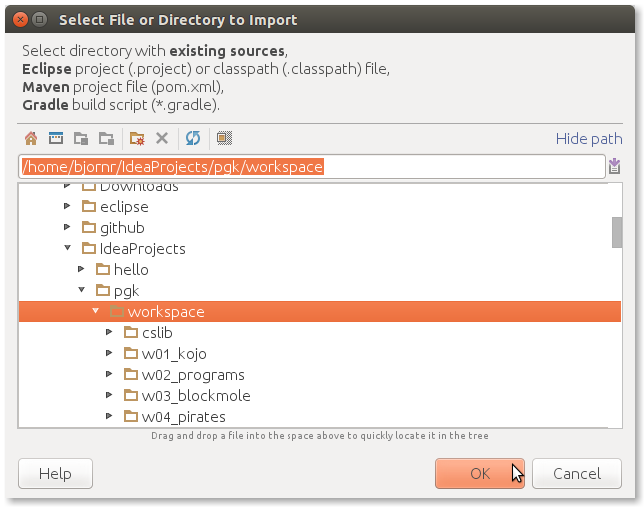
\includegraphics[width=1.0\textwidth]{../img/intellij/idea-import2-select.png}

{\hfill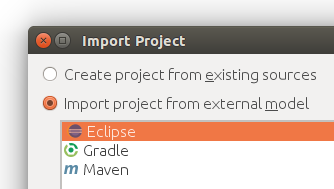
\includegraphics[width=0.4\textwidth]{../img/intellij/idea-import3-eclipse.png}}

\caption{Markera den upp-packade workspace-mappen från zip-filen som du laddat ner från: \url{http://cs.lth.se/pgk/ws} och välj \textbf{Eclipse}-import.}
\label{fig:idea:import23-select}
\end{figure}
}

\begin{figure}
\centering
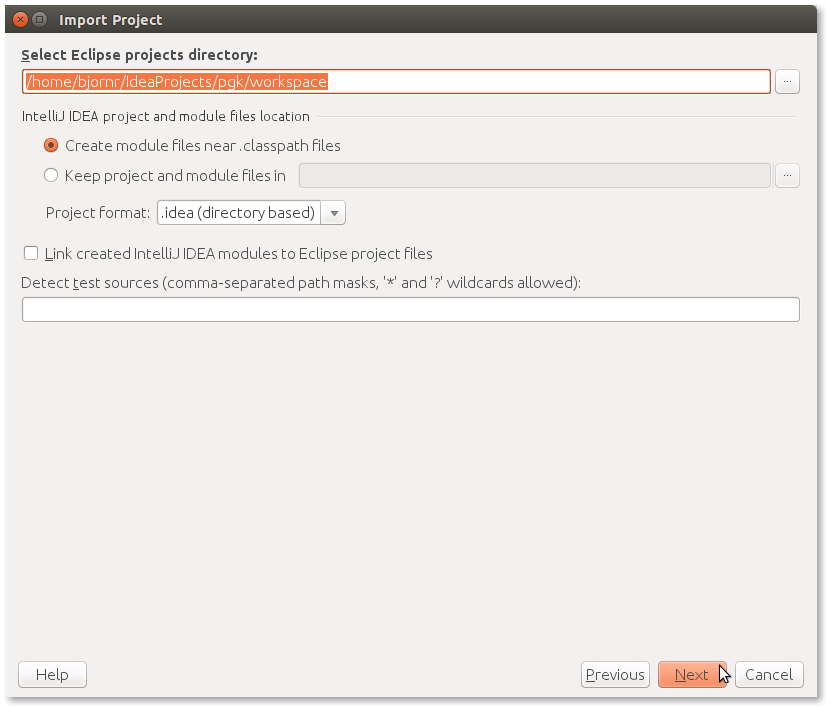
\includegraphics[width=0.85\textwidth]{../img/intellij/idea-import4-directory.png}
\caption{Klicka \Button{Next} med förvalda alternativ oförändrade.}
\label{fig:idea:import4-directory}
\end{figure}

\begin{figure}
\centering
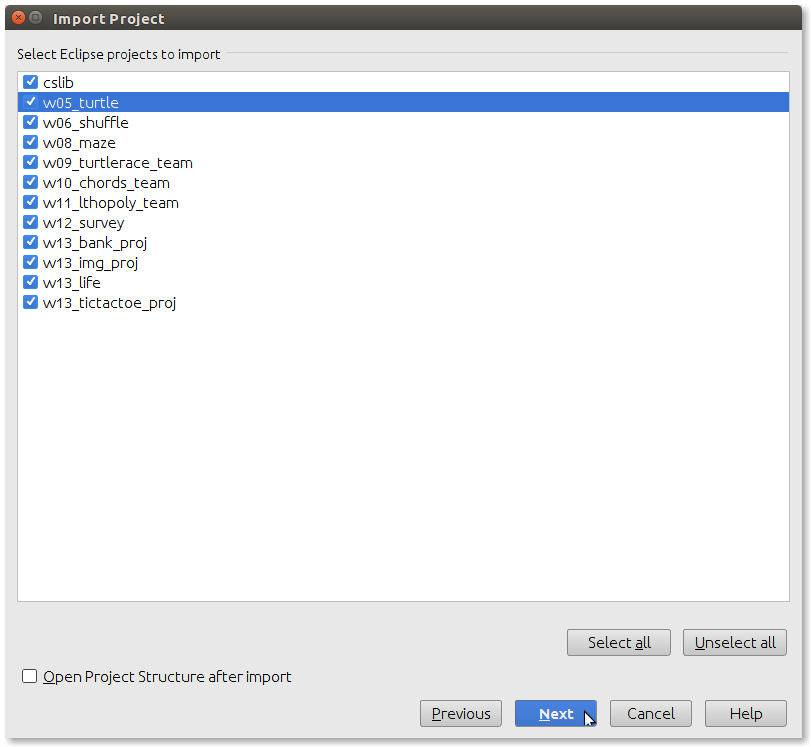
\includegraphics[width=0.85\textwidth]{../img/intellij/idea-import5-select-projects.png}
\caption{Klicka \Button{Next} med alla projekt markerade.}
\label{fig:idea:import5-select-projects}
\end{figure}

\begin{figure}
\centering
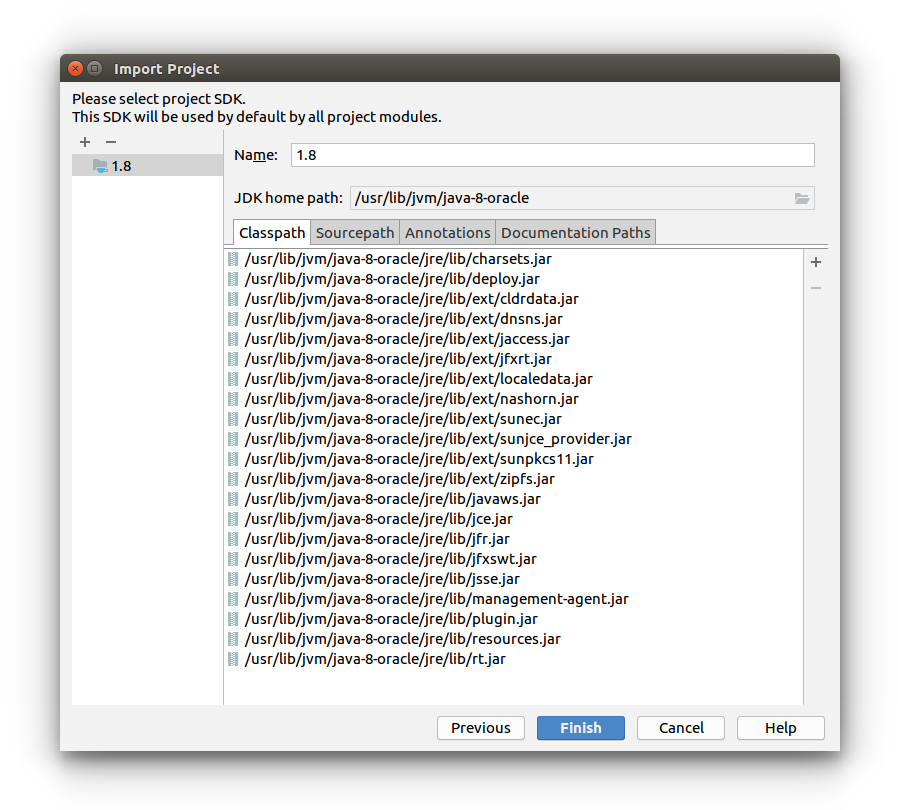
\includegraphics[width=0.8\textwidth]{../img/intellij/idea-import6-select-SDK.png}
\caption{Klicka \Button{Finish} med förifyllda fält oförändrade.}
\label{fig:idea:import6-select-SDK}
\end{figure}

\begin{figure}
\centering
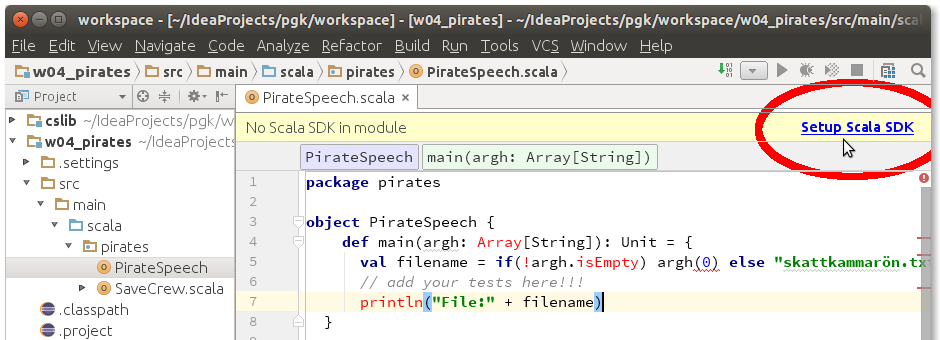
\includegraphics[width=1.0\textwidth]{../img/intellij/idea-import7-setup-scala-sdk.png}

\vspace{1em}{\hfill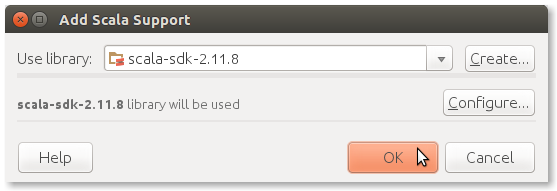
\includegraphics[width=0.6\textwidth]{../img/intellij/idea-import8-add-scala-support.png}}
\caption{Bläddra fram PirateSpeech.scala i projektet \code{w04_pirates} och klicka på länken \textbf{Setup Scala SDK} och klicka \Button{OK} i efterföljande dialog.}
\label{fig:idea:import78-setup-scala-sdk}
\end{figure}

\begin{figure}
\centering
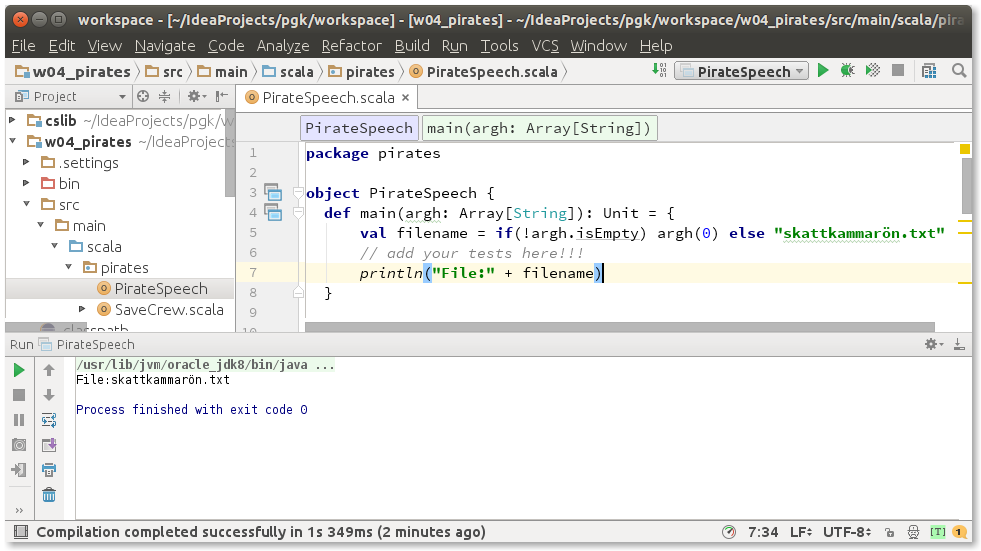
\includegraphics[width=1.0\textwidth]{../img/intellij/idea-import9-run.png}
\caption{Lägg till utskriften i bilden ovan på rad7. Testkör genom att välja menyn \MenuArrow{Run}\Menu{Run..} (eller trycka Alt+Shift+F10) och sedan välja \code{PirateSpeech}. Observera utskriften i utskriftsfönstret.}
\label{fig:idea:import9-run}
\end{figure}

\clearpage

\subsection{Använda debuggern i IntelliJ IDEA med Scala-plugin}

!!! Läs först appendix \ref{appendix:debug}

\subsubsection{Sätta brytpunkter i IntelliJ}\TODO
\subsubsection{Stegad exekvering i IntelliJ}\TODO
\subsubsection{Inspektera variabler i IntelliJ}\TODO
